\begin{exercice*}
    Dans cette figure, les droites qui semblent perpendiculaires ou parallèles le sont réellement. Déterminer :
    \begin{enumerate}
       \item La droite perpendiculaire à (HK) passant par H.
       \item La droite perpendiculaire à (CE) passant par N.
       \item La droite parallèle à (HP) passant par N.
       \item La droite parallèle à (CF) passant par S.
       \item Le droite parallèle à (PN) passant par R.
    \end{enumerate}
    \begin{center}
      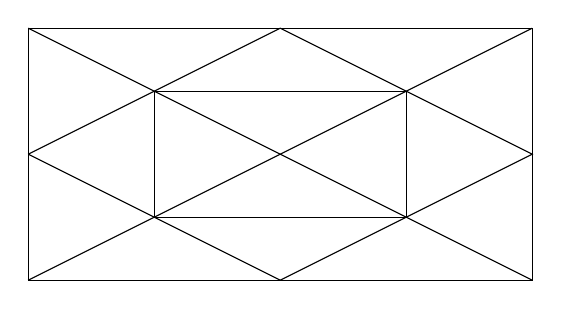
\begin{tikzpicture}[scale=0.8]
         % \draw[help lines, color=black!30, dashed] (0,0) grid (8,4);
         \coordinate (E) at (0,0);
         \coordinate (C) at (4,0);
         \coordinate (F) at (8,0);
         \coordinate (Y) at (2,1);
         \coordinate (P) at (6,1);
         \coordinate (R) at (0,2);
         \coordinate (L) at (4,2);
         \coordinate (N) at (8,2);
         \coordinate (H) at (2,3);
         \coordinate (K) at (6,3);
         \coordinate (D) at (0,4);
         \coordinate (S) at (4,4);
         \coordinate (G) at (8,4);
         \tkzLabelPoints[above](L,H,K,S);
         \tkzLabelPoints[above left](D);
         \tkzLabelPoints[above right](G);
         \tkzLabelPoints[below](C,Y,P);
         \tkzLabelPoints[below left](E);
         \tkzLabelPoints[below right](F);
         \tkzLabelPoints[left](R);
         \tkzLabelPoints[right](N);
         \draw (E)--(F)--(G)--(D)--(E);
         \draw (H)--(Y)--(P)--(K)--(H);
         \draw (D)--(F);
         \draw (E)--(G);
         \draw (R)--(C)--(N)--(S)--(R);
      \end{tikzpicture}
    \end{center}
 \end{exercice*}
\begin{corrige}
Pas de corrigé.
\end{corrige}